\chapter{Proposal Review}\label{C:proposalreview}
Originally proposed was to restrict the function set of neurons to the NAND ($\uparrow$) operations, and construct feedfoward networks with these restricted neurons, however this idea is flawed. Consider the expression p implies q, $p \implies q \iff p \uparrow (q \uparrow q)$.

\begin{figure}[H]
  \centering
  \begin{minipage}[b]{0.6\textwidth}
    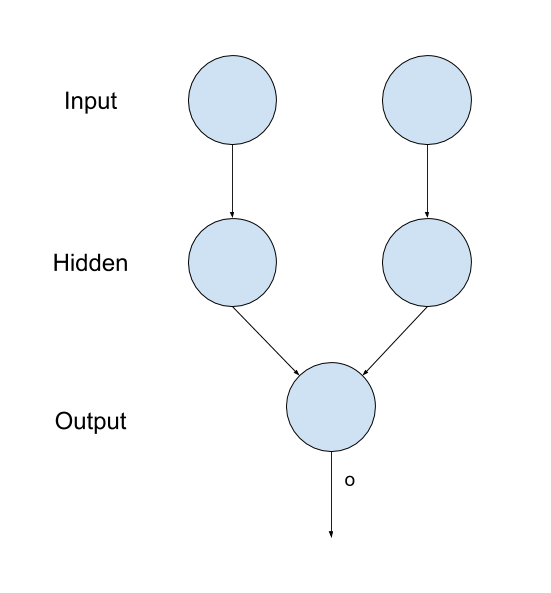
\includegraphics[width=\textwidth]{implys-nand-net.png}
    \caption{}
    \label{fig:implys-nand-net}
  \end{minipage}
  \hfill
\end{figure}

Figure \ref{fig:implys-nand-net} demonstrates the structure a feed-forward network attempting to represent implies would look like. Two inputs and one output, defined by the problem. Two hidden neurons as implies is the NAND of two values, $p$ and $q \uparrow q \iff \lnot q$, consequently the output neuron is computing the NAND of two hidden units. For $o$ to be the output required then one node in the hidden layer would have to act as an identity, passing the input $p$ to the output neuron. NAND cant act as an identity.